\documentclass[twoside]{book}

% Packages required by doxygen
\usepackage{fixltx2e}
\usepackage{calc}
\usepackage{doxygen}
\usepackage[export]{adjustbox} % also loads graphicx
\usepackage{graphicx}
\usepackage[utf8]{inputenc}
\usepackage{makeidx}
\usepackage{multicol}
\usepackage{multirow}
\PassOptionsToPackage{warn}{textcomp}
\usepackage{textcomp}
\usepackage[nointegrals]{wasysym}
\usepackage[table]{xcolor}

% Font selection
\usepackage[T1]{fontenc}
\usepackage[scaled=.90]{helvet}
\usepackage{courier}
\usepackage{amssymb}
\usepackage{sectsty}
\renewcommand{\familydefault}{\sfdefault}
\allsectionsfont{%
  \fontseries{bc}\selectfont%
  \color{darkgray}%
}
\renewcommand{\DoxyLabelFont}{%
  \fontseries{bc}\selectfont%
  \color{darkgray}%
}
\newcommand{\+}{\discretionary{\mbox{\scriptsize$\hookleftarrow$}}{}{}}

% Page & text layout
\usepackage{geometry}
\geometry{%
  a4paper,%
  top=2.5cm,%
  bottom=2.5cm,%
  left=2.5cm,%
  right=2.5cm%
}
\tolerance=750
\hfuzz=15pt
\hbadness=750
\setlength{\emergencystretch}{15pt}
\setlength{\parindent}{0cm}
\setlength{\parskip}{3ex plus 2ex minus 2ex}
\makeatletter
\renewcommand{\paragraph}{%
  \@startsection{paragraph}{4}{0ex}{-1.0ex}{1.0ex}{%
    \normalfont\normalsize\bfseries\SS@parafont%
  }%
}
\renewcommand{\subparagraph}{%
  \@startsection{subparagraph}{5}{0ex}{-1.0ex}{1.0ex}{%
    \normalfont\normalsize\bfseries\SS@subparafont%
  }%
}
\makeatother

% Headers & footers
\usepackage{fancyhdr}
\pagestyle{fancyplain}
\fancyhead[LE]{\fancyplain{}{\bfseries\thepage}}
\fancyhead[CE]{\fancyplain{}{}}
\fancyhead[RE]{\fancyplain{}{\bfseries\leftmark}}
\fancyhead[LO]{\fancyplain{}{\bfseries\rightmark}}
\fancyhead[CO]{\fancyplain{}{}}
\fancyhead[RO]{\fancyplain{}{\bfseries\thepage}}
\fancyfoot[LE]{\fancyplain{}{}}
\fancyfoot[CE]{\fancyplain{}{}}
\fancyfoot[RE]{\fancyplain{}{\bfseries\scriptsize Generated by Doxygen }}
\fancyfoot[LO]{\fancyplain{}{\bfseries\scriptsize Generated by Doxygen }}
\fancyfoot[CO]{\fancyplain{}{}}
\fancyfoot[RO]{\fancyplain{}{}}
\renewcommand{\footrulewidth}{0.4pt}
\renewcommand{\chaptermark}[1]{%
  \markboth{#1}{}%
}
\renewcommand{\sectionmark}[1]{%
  \markright{\thesection\ #1}%
}

% Indices & bibliography
\usepackage{natbib}
\usepackage[titles]{tocloft}
\setcounter{tocdepth}{3}
\setcounter{secnumdepth}{5}
\makeindex

% Hyperlinks (required, but should be loaded last)
\usepackage{ifpdf}
\ifpdf
  \usepackage[pdftex,pagebackref=true]{hyperref}
\else
  \usepackage[ps2pdf,pagebackref=true]{hyperref}
\fi
\hypersetup{%
  colorlinks=true,%
  linkcolor=blue,%
  citecolor=blue,%
  unicode%
}

% Custom commands
\newcommand{\clearemptydoublepage}{%
  \newpage{\pagestyle{empty}\cleardoublepage}%
}

\usepackage{caption}
\captionsetup{labelsep=space,justification=centering,font={bf},singlelinecheck=off,skip=4pt,position=top}

%===== C O N T E N T S =====

\begin{document}

% Titlepage & ToC
\hypersetup{pageanchor=false,
             bookmarksnumbered=true,
             pdfencoding=unicode
            }
\pagenumbering{roman}
\begin{titlepage}
\vspace*{7cm}
\begin{center}%
{\Large My Project }\\
\vspace*{1cm}
{\large Generated by Doxygen 1.8.11}\\
\end{center}
\end{titlepage}
\clearemptydoublepage
\tableofcontents
\clearemptydoublepage
\pagenumbering{arabic}
\hypersetup{pageanchor=true}

%--- Begin generated contents ---
\chapter{Hierarchical Index}
\section{Class Hierarchy}
This inheritance list is sorted roughly, but not completely, alphabetically\+:\begin{DoxyCompactList}
\item \contentsline{section}{keypad}{\pageref{classkeypad}}{}
\item \contentsline{section}{lock}{\pageref{classlock}}{}
\item \contentsline{section}{motor}{\pageref{classmotor}}{}
\item \contentsline{section}{movement}{\pageref{classmovement}}{}
\item \contentsline{section}{P\+W\+M\+\_\+signal}{\pageref{class_p_w_m__signal}}{}
\begin{DoxyCompactList}
\item \contentsline{section}{servo}{\pageref{classservo}}{}
\end{DoxyCompactList}
\item \contentsline{section}{whistle}{\pageref{classwhistle}}{}
\end{DoxyCompactList}

\chapter{Class Index}
\section{Class List}
Here are the classes, structs, unions and interfaces with brief descriptions\+:\begin{DoxyCompactList}
\item\contentsline{section}{\hyperlink{classkeypad}{keypad} \\*Keypad class }{\pageref{classkeypad}}{}
\item\contentsline{section}{\hyperlink{classlock}{lock} \\*Lock class }{\pageref{classlock}}{}
\item\contentsline{section}{\hyperlink{classmotor}{motor} \\*Class for control of 9g\+\_\+servo }{\pageref{classmotor}}{}
\item\contentsline{section}{\hyperlink{classmovement}{movement} \\*Class movement }{\pageref{classmovement}}{}
\item\contentsline{section}{\hyperlink{classpassword}{password} \\*Password A\+DT }{\pageref{classpassword}}{}
\item\contentsline{section}{\hyperlink{classprofile}{profile} \\*Class profile }{\pageref{classprofile}}{}
\item\contentsline{section}{\hyperlink{classpwm}{pwm} \\*Class for pwm signal }{\pageref{classpwm}}{}
\item\contentsline{section}{\hyperlink{class_p_w_m__signal}{P\+W\+M\+\_\+signal} \\*Basic P\+WM signal }{\pageref{class_p_w_m__signal}}{}
\item\contentsline{section}{\hyperlink{classservo}{servo} \\*Servo controll class }{\pageref{classservo}}{}
\item\contentsline{section}{\hyperlink{classsound}{sound} \\*Microphone measure class }{\pageref{classsound}}{}
\item\contentsline{section}{\hyperlink{classsoundlock}{soundlock} \\*Soundlock class }{\pageref{classsoundlock}}{}
\end{DoxyCompactList}

\chapter{File Index}
\section{File List}
Here is a list of all documented files with brief descriptions\+:\begin{DoxyCompactList}
\item\contentsline{section}{{\bfseries admin.\+hpp} }{\pageref{admin_8hpp}}{}
\item\contentsline{section}{{\bfseries keypad.\+hpp} }{\pageref{keypad_8hpp}}{}
\item\contentsline{section}{{\bfseries lock.\+hpp} }{\pageref{lock_8hpp}}{}
\item\contentsline{section}{{\bfseries motor\+\_\+g9.\+hpp} }{\pageref{motor__g9_8hpp}}{}
\item\contentsline{section}{{\bfseries movement.\+hpp} }{\pageref{movement_8hpp}}{}
\item\contentsline{section}{{\bfseries password.\+hpp} }{\pageref{password_8hpp}}{}
\item\contentsline{section}{{\bfseries profile.\+hpp} }{\pageref{profile_8hpp}}{}
\item\contentsline{section}{{\bfseries pwm.\+hpp} }{\pageref{pwm_8hpp}}{}
\item\contentsline{section}{\hyperlink{_p_w_m__signal_8hpp}{P\+W\+M\+\_\+signal.\+hpp} }{\pageref{_p_w_m__signal_8hpp}}{}
\item\contentsline{section}{\hyperlink{servo_8hpp}{servo.\+hpp} }{\pageref{servo_8hpp}}{}
\item\contentsline{section}{{\bfseries sound.\+hpp} }{\pageref{sound_8hpp}}{}
\item\contentsline{section}{{\bfseries sound\+\_\+lock.\+hpp} }{\pageref{sound__lock_8hpp}}{}
\item\contentsline{section}{{\bfseries touchless\+\_\+safe.\+hpp} }{\pageref{touchless__safe_8hpp}}{}
\end{DoxyCompactList}

\chapter{Class Documentation}
\hypertarget{classmotor}{}\section{motor Class Reference}
\label{classmotor}\index{motor@{motor}}


class for control of 9g\+\_\+servo  




{\ttfamily \#include $<$motor\+\_\+g9.\+hpp$>$}

Inheritance diagram for motor\+:\begin{figure}[H]
\begin{center}
\leavevmode
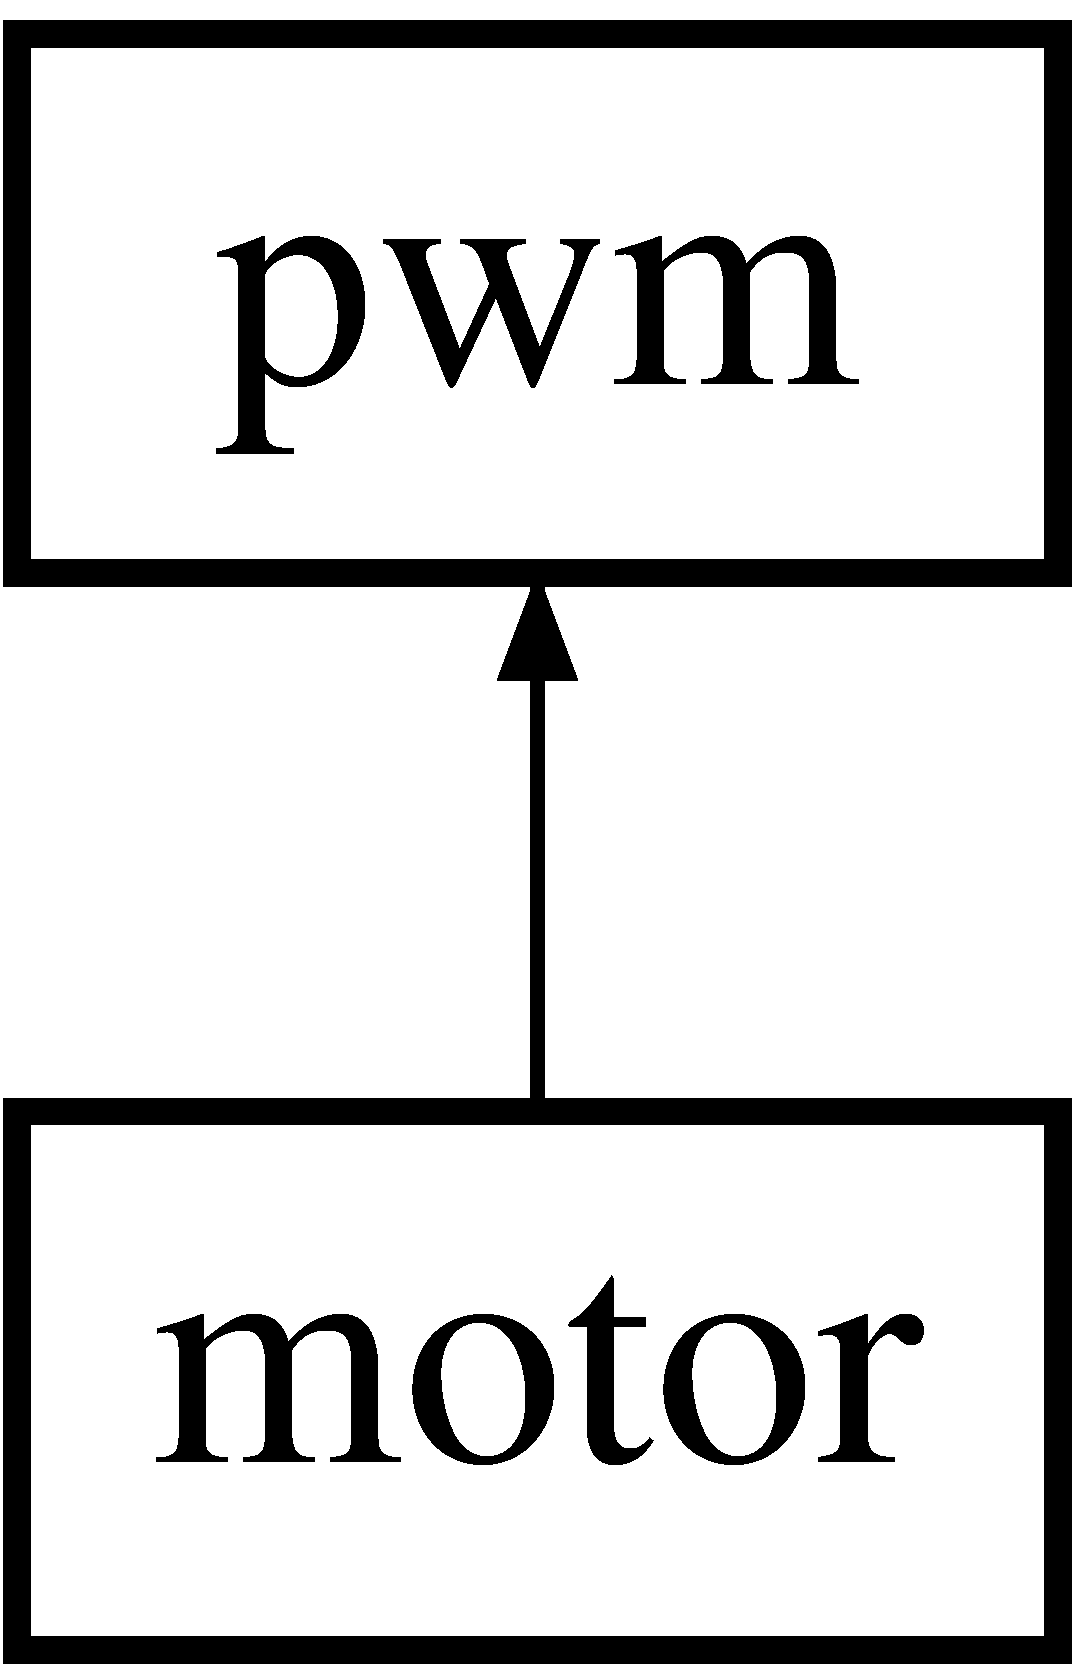
\includegraphics[height=4.000000cm]{classmotor}
\end{center}
\end{figure}
\subsection*{Public Member Functions}
\begin{DoxyCompactItemize}
\item 
\hyperlink{classmotor_a2a03c0b137ceaf886d406f55bc1dfc6d}{motor} (hwlib\+::target\+::pin\+\_\+out \&pwmpin)
\begin{DoxyCompactList}\small\item\em default constructor \end{DoxyCompactList}\item 
void \hyperlink{classmotor_a4d056e4f75a5613ef50a4ae4ed95525d}{turn} (int degrees)
\begin{DoxyCompactList}\small\item\em turn the servo to an desired amount of degrees. \end{DoxyCompactList}\item 
void \hyperlink{classmotor_a942b9474ad3226a035908333d5d09a86}{turnto0} ()
\begin{DoxyCompactList}\small\item\em turnto0 function \end{DoxyCompactList}\item 
void \hyperlink{classmotor_a8983111ce2a6fb60d1ef4d26028981c8}{turnto90} ()
\begin{DoxyCompactList}\small\item\em turnto0 function \end{DoxyCompactList}\end{DoxyCompactItemize}


\subsection{Detailed Description}
class for control of 9g\+\_\+servo 

this class is an decorator class to the pwm class in this class the pulse function is used to create the signal used for the \hyperlink{classservo}{servo( 9g analog)} 

\subsection{Constructor \& Destructor Documentation}
\index{motor@{motor}!motor@{motor}}
\index{motor@{motor}!motor@{motor}}
\subsubsection[{\texorpdfstring{motor(hwlib\+::target\+::pin\+\_\+out \&pwmpin)}{motor(hwlib::target::pin_out &pwmpin)}}]{\setlength{\rightskip}{0pt plus 5cm}motor\+::motor (
\begin{DoxyParamCaption}
\item[{hwlib\+::target\+::pin\+\_\+out \&}]{pwmpin}
\end{DoxyParamCaption}
)}\hypertarget{classmotor_a2a03c0b137ceaf886d406f55bc1dfc6d}{}\label{classmotor_a2a03c0b137ceaf886d406f55bc1dfc6d}


default constructor 

the constructor gets an reference to the ouput pin used for the pwm signal used for the servo 

\subsection{Member Function Documentation}
\index{motor@{motor}!turn@{turn}}
\index{turn@{turn}!motor@{motor}}
\subsubsection[{\texorpdfstring{turn(int degrees)}{turn(int degrees)}}]{\setlength{\rightskip}{0pt plus 5cm}void motor\+::turn (
\begin{DoxyParamCaption}
\item[{int}]{degrees}
\end{DoxyParamCaption}
)}\hypertarget{classmotor_a4d056e4f75a5613ef50a4ae4ed95525d}{}\label{classmotor_a4d056e4f75a5613ef50a4ae4ed95525d}


turn the servo to an desired amount of degrees. 

turn function gets an amount of degrees and calculates the correct value for the wait in the pulse function \index{motor@{motor}!turnto0@{turnto0}}
\index{turnto0@{turnto0}!motor@{motor}}
\subsubsection[{\texorpdfstring{turnto0()}{turnto0()}}]{\setlength{\rightskip}{0pt plus 5cm}void motor\+::turnto0 (
\begin{DoxyParamCaption}
{}
\end{DoxyParamCaption}
)}\hypertarget{classmotor_a942b9474ad3226a035908333d5d09a86}{}\label{classmotor_a942b9474ad3226a035908333d5d09a86}


turnto0 function 

this function uses the turn function and is pre set to turn the servo to 0 degrees in contrast to the turnto90 function \index{motor@{motor}!turnto90@{turnto90}}
\index{turnto90@{turnto90}!motor@{motor}}
\subsubsection[{\texorpdfstring{turnto90()}{turnto90()}}]{\setlength{\rightskip}{0pt plus 5cm}void motor\+::turnto90 (
\begin{DoxyParamCaption}
{}
\end{DoxyParamCaption}
)}\hypertarget{classmotor_a8983111ce2a6fb60d1ef4d26028981c8}{}\label{classmotor_a8983111ce2a6fb60d1ef4d26028981c8}


turnto0 function 

this function uses the turn function and is pre set to turn the servo to 90 degree in contrast to the turnto0 function 

The documentation for this class was generated from the following files\+:\begin{DoxyCompactItemize}
\item 
motor\+\_\+g9.\+hpp\item 
motor\+\_\+g9.\+cpp\end{DoxyCompactItemize}

\hypertarget{class_p_w_m__signal}{}\section{P\+W\+M\+\_\+signal Class Reference}
\label{class_p_w_m__signal}\index{P\+W\+M\+\_\+signal@{P\+W\+M\+\_\+signal}}


Basic P\+WM signal.  




{\ttfamily \#include $<$P\+W\+M\+\_\+signal.\+hpp$>$}

Inheritance diagram for P\+W\+M\+\_\+signal\+:\begin{figure}[H]
\begin{center}
\leavevmode
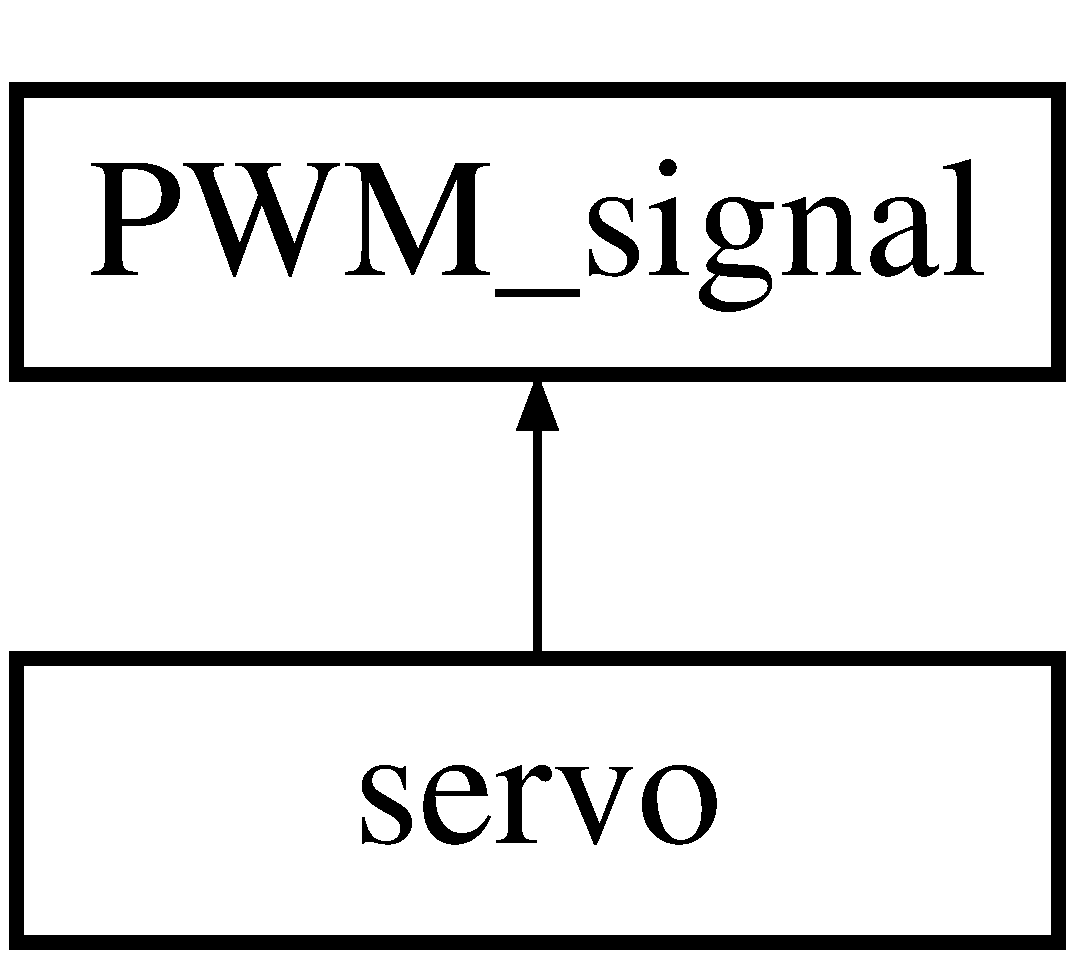
\includegraphics[height=2.000000cm]{class_p_w_m__signal}
\end{center}
\end{figure}
\subsection*{Public Member Functions}
\begin{DoxyCompactItemize}
\item 
\hyperlink{class_p_w_m__signal_ad64aad0e6fe9cf246715bc9cf0f78247}{P\+W\+M\+\_\+signal} (hwlib\+::target\+::pin\+\_\+out \&pwm\+Pin)
\begin{DoxyCompactList}\small\item\em Default constructor. \end{DoxyCompactList}\item 
virtual void \hyperlink{class_p_w_m__signal_a82a9e4648b24a15992b59918e640157c}{P\+W\+M\+\_\+pulse} (int pulse\+Width)
\begin{DoxyCompactList}\small\item\em One pulse. \end{DoxyCompactList}\end{DoxyCompactItemize}


\subsection{Detailed Description}
Basic P\+WM signal. 

This class is for creating a basic P\+WN signal object and then call seperate pules with a certain pulsewidth. 

\subsection{Constructor \& Destructor Documentation}
\index{P\+W\+M\+\_\+signal@{P\+W\+M\+\_\+signal}!P\+W\+M\+\_\+signal@{P\+W\+M\+\_\+signal}}
\index{P\+W\+M\+\_\+signal@{P\+W\+M\+\_\+signal}!P\+W\+M\+\_\+signal@{P\+W\+M\+\_\+signal}}
\subsubsection[{\texorpdfstring{P\+W\+M\+\_\+signal(hwlib\+::target\+::pin\+\_\+out \&pwm\+Pin)}{PWM_signal(hwlib::target::pin_out &pwmPin)}}]{\setlength{\rightskip}{0pt plus 5cm}P\+W\+M\+\_\+signal\+::\+P\+W\+M\+\_\+signal (
\begin{DoxyParamCaption}
\item[{hwlib\+::target\+::pin\+\_\+out \&}]{pwm\+Pin}
\end{DoxyParamCaption}
)}\hypertarget{class_p_w_m__signal_ad64aad0e6fe9cf246715bc9cf0f78247}{}\label{class_p_w_m__signal_ad64aad0e6fe9cf246715bc9cf0f78247}


Default constructor. 

This constructor sets up a pin to control using pwm. It does this using the pin\+\_\+out class in namespace hwlib. 

\subsection{Member Function Documentation}
\index{P\+W\+M\+\_\+signal@{P\+W\+M\+\_\+signal}!P\+W\+M\+\_\+pulse@{P\+W\+M\+\_\+pulse}}
\index{P\+W\+M\+\_\+pulse@{P\+W\+M\+\_\+pulse}!P\+W\+M\+\_\+signal@{P\+W\+M\+\_\+signal}}
\subsubsection[{\texorpdfstring{P\+W\+M\+\_\+pulse(int pulse\+Width)}{PWM_pulse(int pulseWidth)}}]{\setlength{\rightskip}{0pt plus 5cm}void P\+W\+M\+\_\+signal\+::\+P\+W\+M\+\_\+pulse (
\begin{DoxyParamCaption}
\item[{int}]{pulse\+Width}
\end{DoxyParamCaption}
)\hspace{0.3cm}{\ttfamily [virtual]}}\hypertarget{class_p_w_m__signal_a82a9e4648b24a15992b59918e640157c}{}\label{class_p_w_m__signal_a82a9e4648b24a15992b59918e640157c}


One pulse. 

This function is made to create one P\+WM pulse with a user specified pulsewidth. The wait time between every pulse is about 20 ms. 

The documentation for this class was generated from the following files\+:\begin{DoxyCompactItemize}
\item 
\hyperlink{_p_w_m__signal_8hpp}{P\+W\+M\+\_\+signal.\+hpp}\item 
P\+W\+M\+\_\+signal.\+cpp\end{DoxyCompactItemize}

\hypertarget{classservo}{}\section{servo Class Reference}
\label{classservo}\index{servo@{servo}}


Servo controll class.  




{\ttfamily \#include $<$servo.\+hpp$>$}

Inheritance diagram for servo\+:\begin{figure}[H]
\begin{center}
\leavevmode
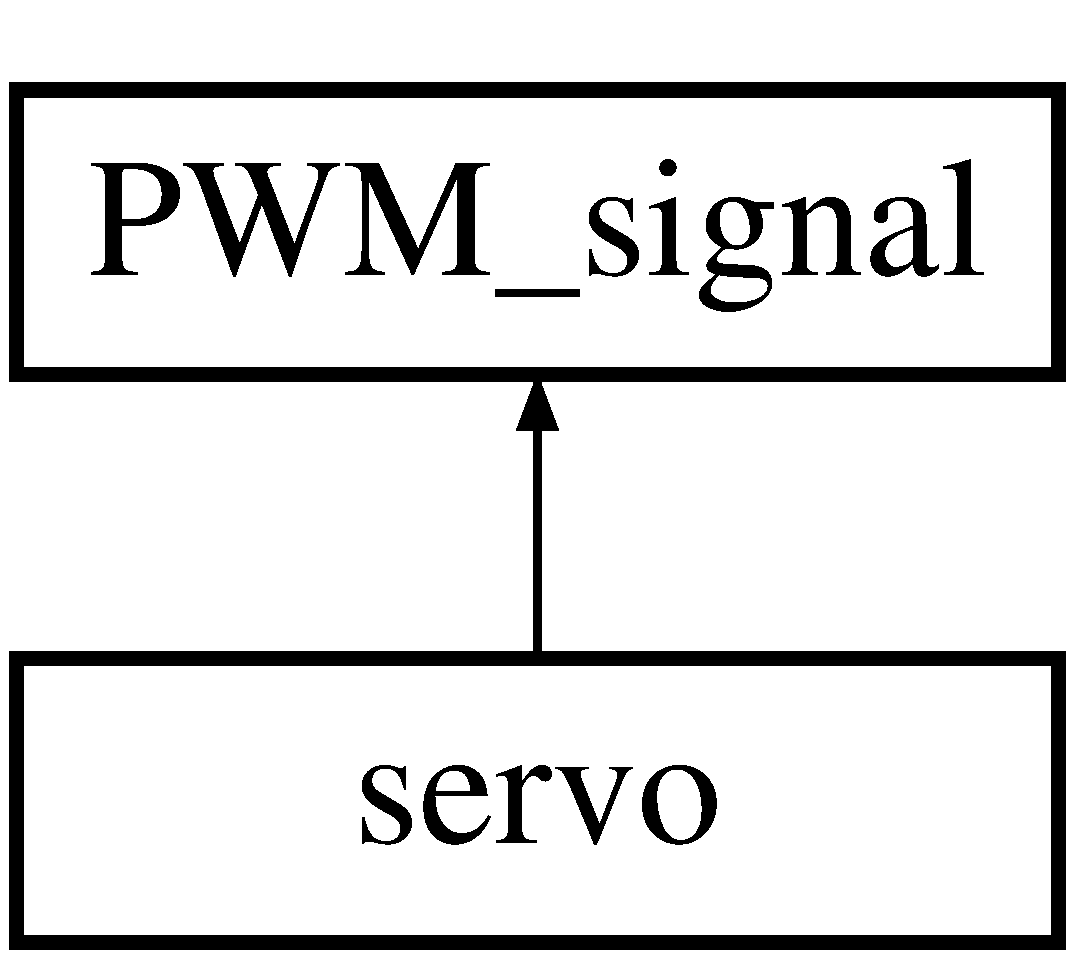
\includegraphics[height=2.000000cm]{classservo}
\end{center}
\end{figure}
\subsection*{Public Member Functions}
\begin{DoxyCompactItemize}
\item 
\hyperlink{classservo_a99c6a39c75cd91b8b2c498cca77d7239}{servo} (hwlib\+::target\+::pin\+\_\+out \&pwm\+Pin)
\begin{DoxyCompactList}\small\item\em Default constructor. \end{DoxyCompactList}\item 
void \hyperlink{classservo_ac0fa39642e5294471844d1fd56e9fec5}{turn\+Degrees} (int degrees)
\begin{DoxyCompactList}\small\item\em Turn the servo to a amount of degrees. \end{DoxyCompactList}\end{DoxyCompactItemize}


\subsection{Detailed Description}
Servo controll class. 

This class is meant to act as a decorator class to the \hyperlink{class_p_w_m__signal}{P\+W\+M\+\_\+signal} class. The idea is that it takes the pulse function and modifies it to send the correct signal for a servo. 

\subsection{Constructor \& Destructor Documentation}
\index{servo@{servo}!servo@{servo}}
\index{servo@{servo}!servo@{servo}}
\subsubsection[{\texorpdfstring{servo(hwlib\+::target\+::pin\+\_\+out \&pwm\+Pin)}{servo(hwlib::target::pin_out &pwmPin)}}]{\setlength{\rightskip}{0pt plus 5cm}servo\+::servo (
\begin{DoxyParamCaption}
\item[{hwlib\+::target\+::pin\+\_\+out \&}]{pwm\+Pin}
\end{DoxyParamCaption}
)}\hypertarget{classservo_a99c6a39c75cd91b8b2c498cca77d7239}{}\label{classservo_a99c6a39c75cd91b8b2c498cca77d7239}


Default constructor. 

This constructor gets a reference to the already existing P\+WM signal taken from the \hyperlink{class_p_w_m__signal}{P\+W\+M\+\_\+signal} class. 

\subsection{Member Function Documentation}
\index{servo@{servo}!turn\+Degrees@{turn\+Degrees}}
\index{turn\+Degrees@{turn\+Degrees}!servo@{servo}}
\subsubsection[{\texorpdfstring{turn\+Degrees(int degrees)}{turnDegrees(int degrees)}}]{\setlength{\rightskip}{0pt plus 5cm}void servo\+::turn\+Degrees (
\begin{DoxyParamCaption}
\item[{int}]{degrees}
\end{DoxyParamCaption}
)}\hypertarget{classservo_ac0fa39642e5294471844d1fd56e9fec5}{}\label{classservo_ac0fa39642e5294471844d1fd56e9fec5}


Turn the servo to a amount of degrees. 

This function get an amount of degrees and then it calculates the wait time. This wait time is beeing given to the pulse function. It also makes sure the servo gets more then one pulse to make sure it has enough time to turn to the set amount of degrees. 

The documentation for this class was generated from the following files\+:\begin{DoxyCompactItemize}
\item 
\hyperlink{servo_8hpp}{servo.\+hpp}\item 
servo.\+cpp\end{DoxyCompactItemize}

\chapter{File Documentation}
\hypertarget{_p_w_m__signal_8hpp}{}\section{P\+W\+M\+\_\+signal.\+hpp File Reference}
\label{_p_w_m__signal_8hpp}\index{P\+W\+M\+\_\+signal.\+hpp@{P\+W\+M\+\_\+signal.\+hpp}}
{\ttfamily \#include \char`\"{}hwlib.\+hpp\char`\"{}}\\*
\subsection*{Classes}
\begin{DoxyCompactItemize}
\item 
class \hyperlink{class_p_w_m__signal}{P\+W\+M\+\_\+signal}
\begin{DoxyCompactList}\small\item\em Basic P\+WM signal. \end{DoxyCompactList}\end{DoxyCompactItemize}

\hypertarget{servo_8hpp}{}\section{servo.\+hpp File Reference}
\label{servo_8hpp}\index{servo.\+hpp@{servo.\+hpp}}
{\ttfamily \#include \char`\"{}P\+W\+M\+\_\+signal.\+hpp\char`\"{}}\\*
{\ttfamily \#include \char`\"{}hwlib.\+hpp\char`\"{}}\\*
\subsection*{Classes}
\begin{DoxyCompactItemize}
\item 
class \hyperlink{classservo}{servo}
\begin{DoxyCompactList}\small\item\em Servo controll class. \end{DoxyCompactList}\end{DoxyCompactItemize}
\subsection*{Macros}
\begin{DoxyCompactItemize}
\item 
\#define {\bfseries M\+A\+X\+\_\+\+D\+E\+G\+R\+E\+ES}~360\hypertarget{servo_8hpp_a4ba510f21f53f375dd98267c4a644281}{}\label{servo_8hpp_a4ba510f21f53f375dd98267c4a644281}

\item 
\#define {\bfseries M\+I\+N\+\_\+\+D\+E\+G\+R\+E\+ES}~0\hypertarget{servo_8hpp_a0433cf7215e086e910d2fc9f84c25e79}{}\label{servo_8hpp_a0433cf7215e086e910d2fc9f84c25e79}

\end{DoxyCompactItemize}

%--- End generated contents ---

% Index
\backmatter
\newpage
\phantomsection
\clearemptydoublepage
\addcontentsline{toc}{chapter}{Index}
\printindex

\end{document}
